\documentclass[amsmath,amssymb,superscriptaddress]{revtex4-1}

\usepackage{graphicx}% Include figure files
\usepackage{dcolumn}% Align table columns on decimal point
\usepackage{bm}% bold math
\usepackage[detect-all]{siunitx}
\usepackage{hyperref}% add hypertext capabilities
\usepackage{xr}
\usepackage{mhchem}
\renewcommand{\thefigure}{S\arabic{figure}}
\renewcommand{\theequation}{S\arabic{equation}}
\renewcommand{\thesection}{S\arabic{section}}
\renewcommand{\thetable}{S\Roman{table}}

\graphicspath{{./figures/}}

\begin{document}                  % DO NOT DELETE THIS LINE

\title{SI for ``Applying molecular simulation to the analysis of lipid monolayer reflectometry''}

\author{A.~R. McCluskey}
\email{a.r.mccluskey@bath.ac.uk}
\affiliation{Department of Chemistry, University of Bath, Claverton Down,
Bath, BA2 7AY, UK}
\affiliation{Diamond Light Source, Harwell Campus, Didcot, OX11 0DE, UK}

\author{J. Grant}
\affiliation{Computing Services, University of Bath, Claverton Down, Bath, BA2 7AY, UK}

\author{A. J. Smith}
\affiliation{Diamond Light Source, Harwell Campus, Didcot, OX11 0DE, UK}

\author{J. L. Rawle}
\affiliation{Diamond Light Source, Harwell Campus, Didcot, OX11 0DE, UK}

\author{D. J. Barlow}
\affiliation{Institute of Pharmaceutical Science, King's College London, London, SE1 9NH, UK}

\author{M. J. Lawrence}
\affiliation{Division of Pharmacy and Optometry, University of Manchester, Manchester, M13 9PT, UK}

\author{S.~C. Parker}
\affiliation{Department of Chemistry, University of Bath, Claverton Down,
Bath, BA2 7AY, UK}

\author{K.~J. Edler}
\email{k.edler@bath.ac.uk}
\affiliation{Department of Chemistry, University of Bath, Claverton Down,
Bath, BA2 7AY, UK}

\date{\today}

\maketitle                        % DO NOT DELETE THIS LINE

This Supplementary Information document is only part of a fully reproducible analysis workflow. The complete workflow, along with all datasets, figure files, and analysis/plotting scripts is available at \url{https://github.com/arm61/sim_vs_trad} (DOI: 10.5281/zenodo.xxxxxxx) under a CC BY-SA 4.0 license.


\section{Abel\`{e}s matrix formalism}

The Abel\`{e}s matrix formalism method invoked the use of the chemically-consistent monolayer model.
For this it is necessary to have the scattering length of the individual head and tail components of the different lipid contrasts, these are given in Table \ref{tab:scat}.
%
\begin{table}[h]
\small
  \caption{\ The different scattering lengths of the head and tail lipid components. }
  \label{tab:scat}
  \begin{tabular*}{0.48\textwidth}{@{\extracolsep{\fill}}lllll}
    \hline
    Contrast & d$_{13}$-DSPC & d$_{70}$-DSPC & d$_{83}$-DSPC & h-DSPC  \\
    \hline
    $b_{\text{head}}$\SI{10e-4}{\angstrom} & 19.54 & 11.21 & 24.75 & 6.01 \\
    $b_{\text{tail}}$\SI{10e-4}{\angstrom} & -3.58 & 69.32 & 69.32 & -3.58 \\
    \hline
  \end{tabular*}
\end{table}
%

In order to apply the Abel\`{e}s matrix formalism, the SLD for the layers, $N$, were determined as detailed in the text of the paper.
This $\text{SLD}_N$ allows for the determination of the wavevector, $k_N$ at a particular $q$-vector in the $N$-th layer, by considering the difference in SLD between the layer $N$ and the semi-infinite layer 0 (Figure 1),
%
\begin{equation}
	k_N^2 = k_0^2 - 4\pi(\text{SLD}_N - \text{SLD}_0)
\end{equation}
%
where $k_0 = q/2$ and $\text{SLD}_0$ is the SLD of the superphase.
For each of the interfaces between two layers, it is possible to evaluate a Fresnel coefficient, $r_{N,N+1}$, which describes the refraction of the probing radiation occuring between the layers $N$ and $N+1$,
%
\begin{equation}
	r_{N,N+1} = \frac{k_N - k_{N+1}}{k_N + k_{N+1}}\exp{(-2k_Nk_{N+1}\sigma^2_{N, N+1})}.
\end{equation}
%
The exponential factor is due to the fact that the layer is unlikely to be perfectly smooth and will therefore have some roughness, this is modelled as an error function with some width $\sigma_{N,N+1}$ \cite{nevot_caracterisation_1980}.
A phase factor, $\beta_N$, which considers the layer thickness, $d_N$, and the wavevector can then be found,
%
\begin{equation}
	\beta_N =
	\begin{cases}
		0 + 0i & N = 0, \\
		k_N d_N & N > 0.
	\end{cases}
\end{equation}
%
These two parameters are then brought together in the characteristic matrix for the layer, $C_N$,
%
\begin{equation}
	C_N =
	\begin{bmatrix}
		\exp{\beta_N} & r_{N,N+1} \exp{\beta_N} \\
		r_{N,N+1}\exp{-\beta_N} & \exp{-\beta_N}
	\end{bmatrix},
\end{equation}
%
the product sum of which gives a resultant matrix for each value of $q$,
%
\begin{equation}
	M(q) = \prod_{n=0}^{n_{\text{max}}} C_N.
\end{equation}
%
From this matrix, the reflected intensity, $R(q)$, can be determined,
%
\begin{equation}
	R(q) = \frac{|M(q)_{21}|}{|M(q)_{11}|}.
\end{equation}
%

\section{MARTINI potential model considerations}
It was noted in the work of Koutsioubas \cite{koutsioubas_combined_2016}, that the use of the MARTINI water bead, could result in the ordering of the water structure.
This can be observed in the scattering length density profile (Figure \ref{fig:mart}) when the layer thickness of \SI{1}{\angstrom} was used.
In an effort to reduce this effect, a larger layer thickness, or \SI{4}{\angstrom} was used for the MARTINI potential model.
%
\begin{figure*}
 \centering
 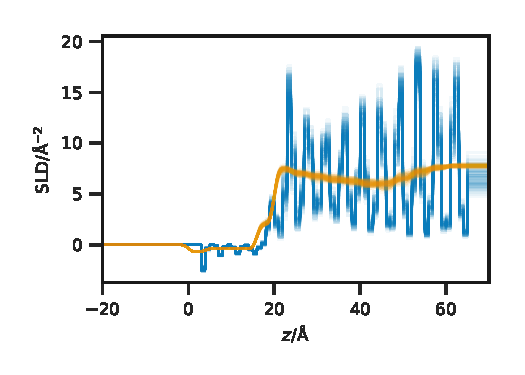
\includegraphics[width=0.49\textwidth]{martiniorder}
 \caption{The scattering length density profile from the MARTINI simulation, at an effective surface pressure of \SI{30}{\milli\newton\per\meter} with a layer thickness of \SI{1}{\angstrom} (blue) and \SI{4}{\angstrom} (orange). }
 \label{fig:mart}
\end{figure*}
%

A negative effect of this large layer thickness, was that the smoothness associated with the \SI{1}{\angstrom} layer was lost.
In an effort to reproduce this, an interfacial roughness of \SI{0.8}{\angstrom} (\SI{20}{\percent} of the layer thickness) was included in the model.
We believe that this gave the MARTINI potential model a fair chance to reproduce the experimental data.
However, as is noted in the main text of the paper, the systematic beading problem lead to more severe issues.

\section{Reflectometry profiles}
Figures \ref{fig:sp20} through \ref{fig:sp50} show the reflectometry profiles for each of the analysis methods that correspond to surface pressures of \SI{20}{\milli\newton\per\meter}, \SI{40}{\milli\newton\per\meter}, and \SI{50}{\milli\newton\per\meter}.
The profile that corresponds to a surface pressure of \SI{30}{\milli\newton\per\meter} is given in Figure 4.
%
\begin{figure*}
 \centering
 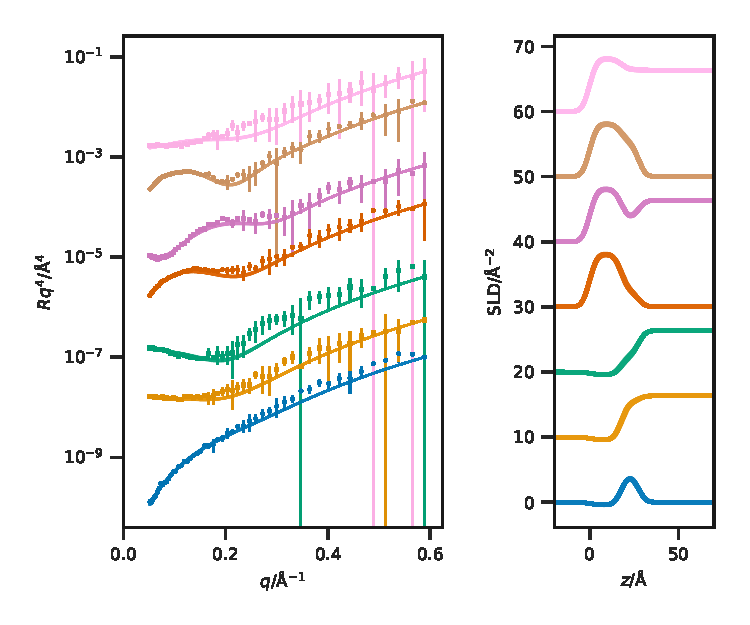
\includegraphics[width=0.49\textwidth]{trad_20}
 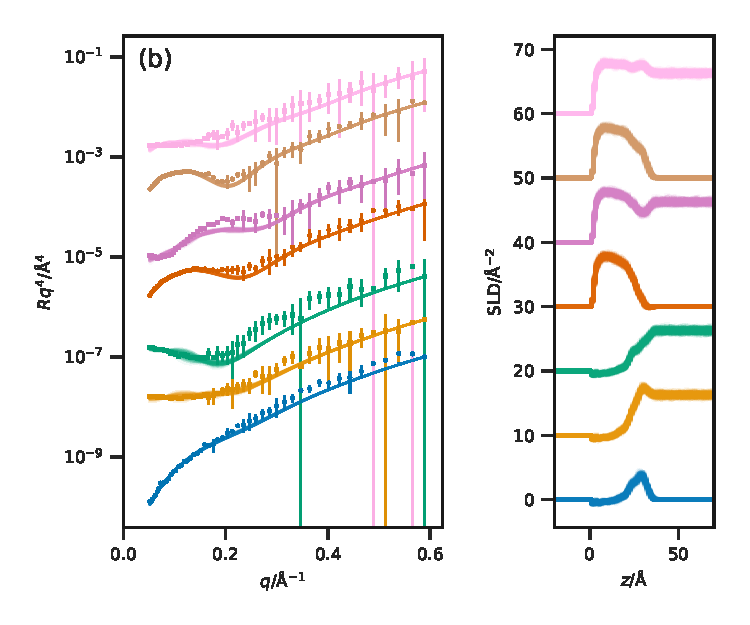
\includegraphics[width=0.49\textwidth]{sim_slipids_20} \\
 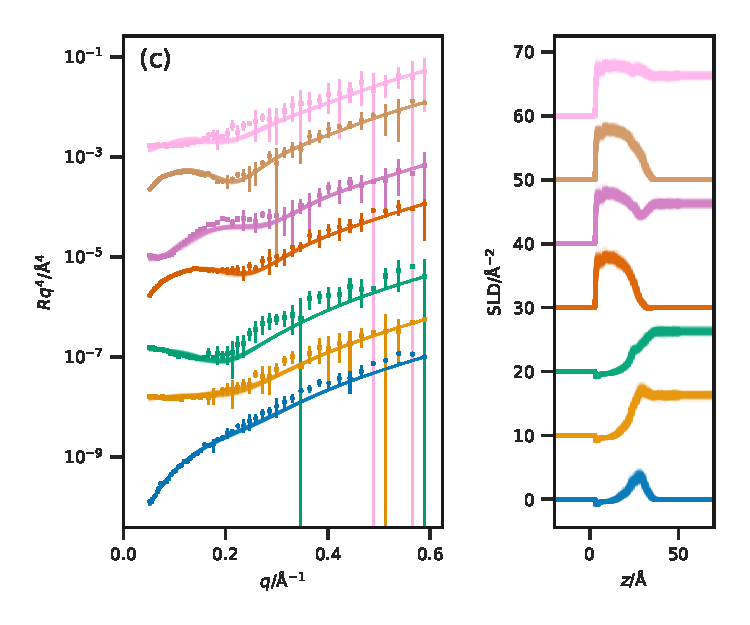
\includegraphics[width=0.49\textwidth]{sim_berger_20}
 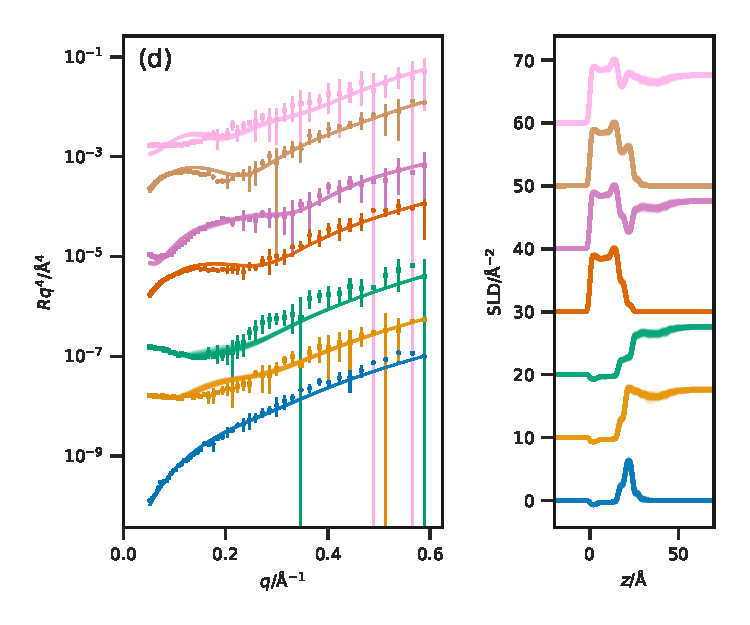
\includegraphics[width=0.49\textwidth]{sim_martini_20}
 \caption{A comparison of the reflectometry and SLD profiles obtained from (a) the monolayer model, (b) the Slipid simulation, (c) the Berger force-force simulation, and (d) the MARTINI potential model simulation at a surface pressure of \SI{20}{\milli\newton\per\meter}. From top-to-bottom the contrasts are as follows; \ce{d_{83}}-\ce{D2O}, \ce{d_{83}}-ACMW, \ce{d_{70}}-\ce{D2O}, \ce{d_{70}}-ACMW, h-\ce{D2O}, \ce{d_{13}}-\ce{D2O}, \ce{d_{13}}-ACMW. The different contrast reflectometry profiles have been offset in the \emph{y}-axis by an order of magnitude and the SLD profiles offset in the \emph{y}-axis by \SI{1e-6}{\per\square\angstrom}, for clarity.}
 \label{fig:sp20}
\end{figure*}
%
%
\begin{figure*}
 \centering
 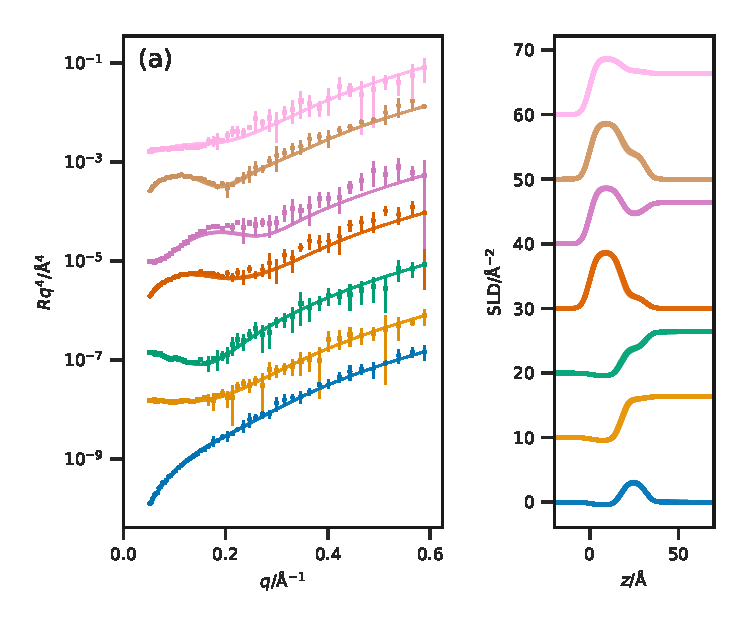
\includegraphics[width=0.49\textwidth]{trad_40}
 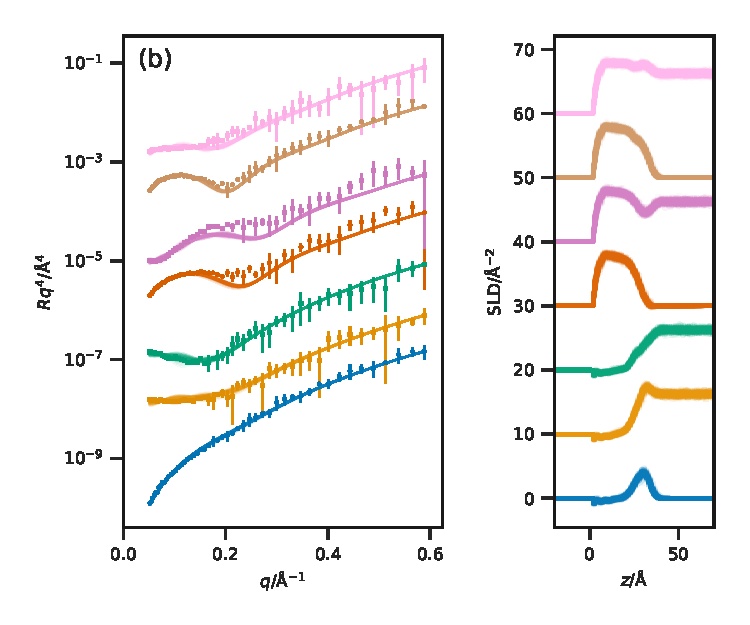
\includegraphics[width=0.49\textwidth]{sim_slipids_40} \\
 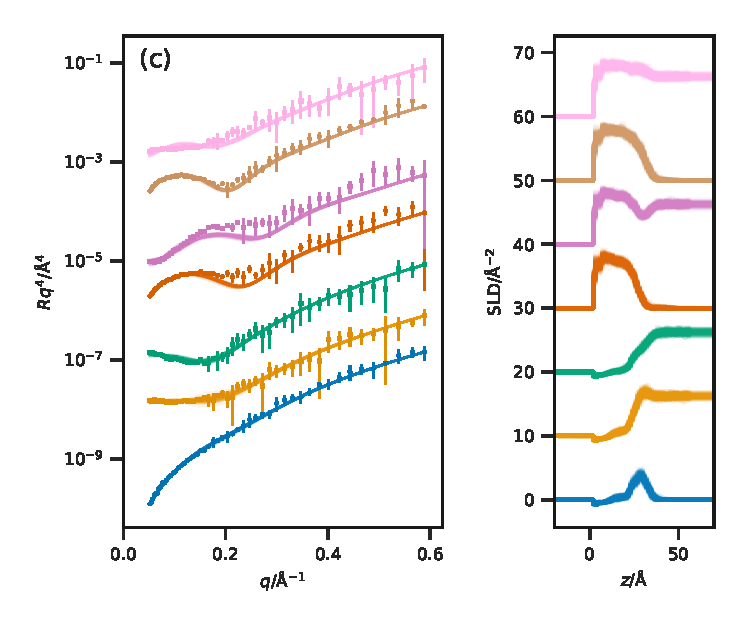
\includegraphics[width=0.49\textwidth]{sim_berger_40}
 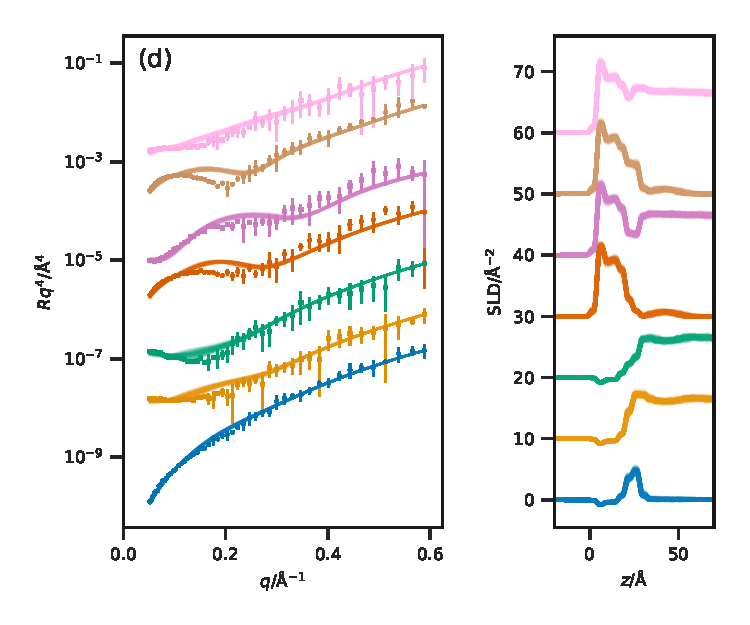
\includegraphics[width=0.49\textwidth]{sim_martini_40}
 \caption{A comparison of the reflectometry and SLD profiles obtained from (a) the monolayer model, (b) the Slipid simulation, (c) the Berger force-force simulation, and (d) the MARTINI potential model simulation at a surface pressure of \SI{40}{\milli\newton\per\meter}. From top-to-bottom the contrasts are as follows; \ce{d_{83}}-\ce{D2O}, \ce{d_{83}}-ACMW, \ce{d_{70}}-\ce{D2O}, \ce{d_{70}}-ACMW, h-\ce{D2O}, \ce{d_{13}}-\ce{D2O}, \ce{d_{13}}-ACMW. The different contrast reflectometry profiles have been offset in the \emph{y}-axis by an order of magnitude and the SLD profiles offset in the \emph{y}-axis by \SI{1e-6}{\per\square\angstrom}, for clarity.}
 \label{fig:sp40}
\end{figure*}
%
%
\begin{figure*}
 \centering
 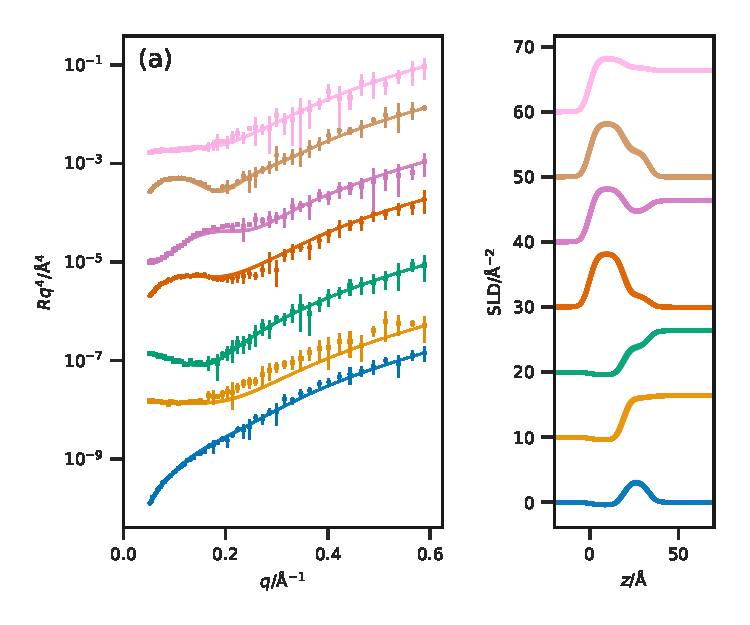
\includegraphics[width=0.49\textwidth]{trad_50}
 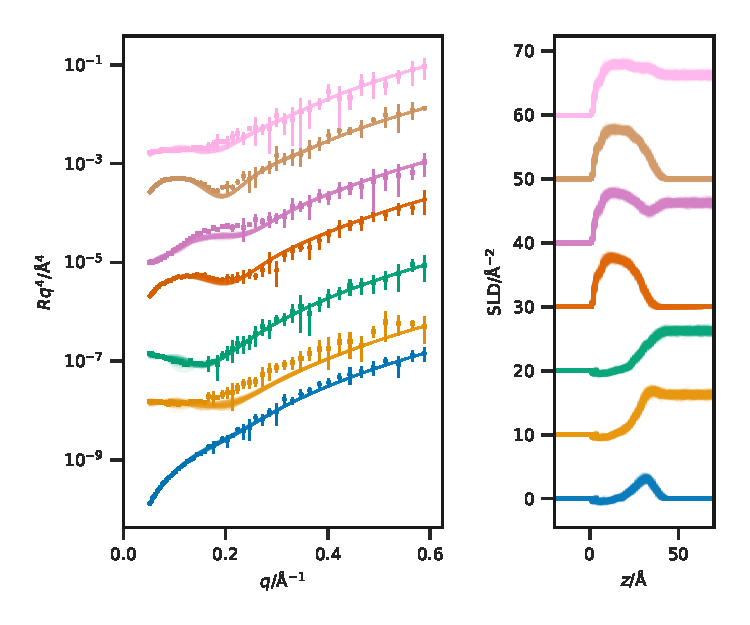
\includegraphics[width=0.49\textwidth]{sim_slipids_50} \\
 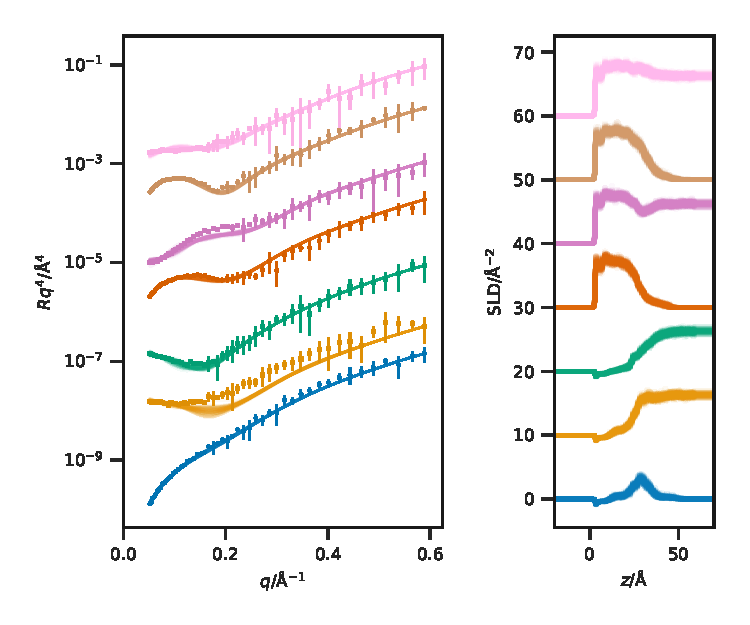
\includegraphics[width=0.49\textwidth]{sim_berger_50}
 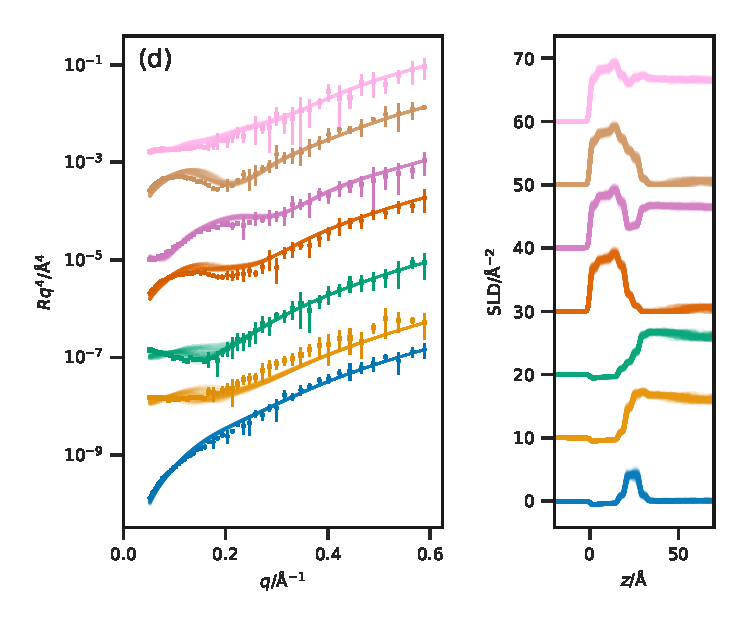
\includegraphics[width=0.49\textwidth]{sim_martini_50}
 \caption{A comparison of the reflectometry and SLD profiles obtained from (a) the monolayer model, (b) the Slipid simulation, (c) the Berger force-force simulation, and (d) the MARTINI potential model simulation at a surface pressure of \SI{50}{\milli\newton\per\meter}. From top-to-bottom the contrasts are as follows; \ce{d_{83}}-\ce{D2O}, \ce{d_{83}}-ACMW, \ce{d_{70}}-\ce{D2O}, \ce{d_{70}}-ACMW, h-\ce{D2O}, \ce{d_{13}}-\ce{D2O}, \ce{d_{13}}-ACMW. The different contrast reflectometry profiles have been offset in the \emph{y}-axis by an order of magnitude and the SLD profiles offset in the \emph{y}-axis by \SI{1e-6}{\per\square\angstrom}, for clarity.}
 \label{fig:sp50}
\end{figure*}
%

\section{Probability distribution functions}
Figures \ref{fig:sl20} to \ref{fig:ma50} show the probability distribution functions for each of the four parametric outcomes from the simulations.
%
\begin{figure*}
 \centering
 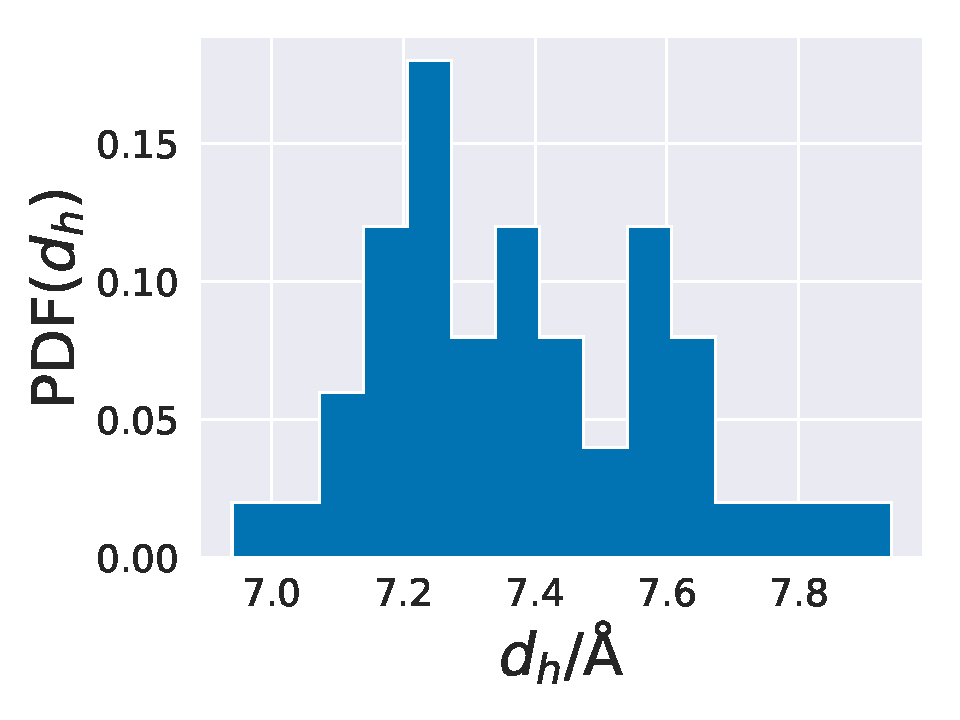
\includegraphics[width=0.32\textwidth]{slipids_20_dh}
 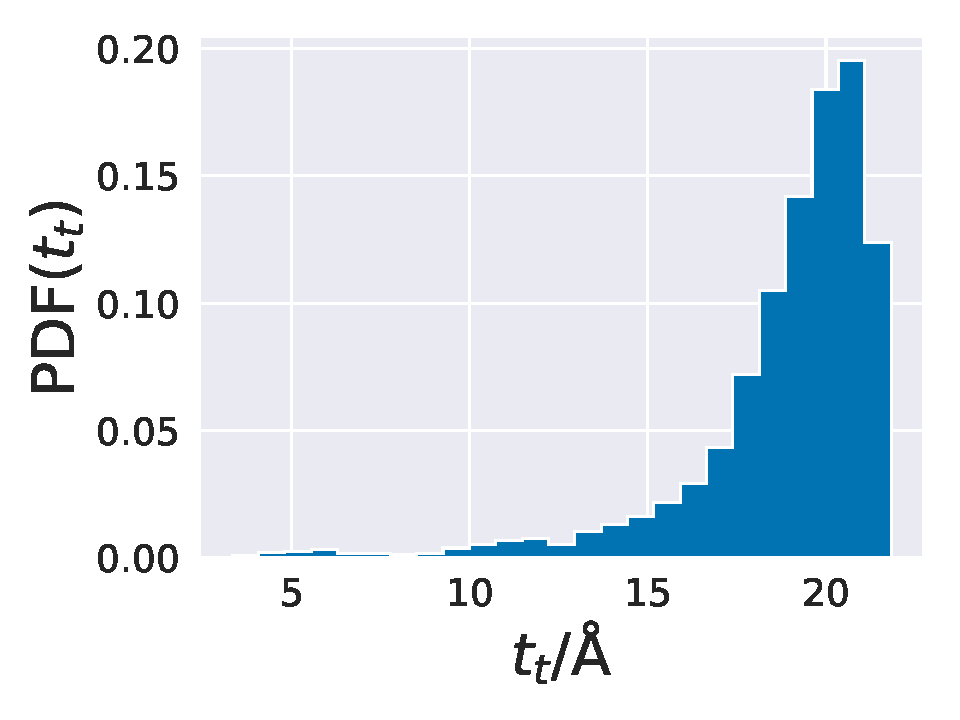
\includegraphics[width=0.32\textwidth]{slipids_20_tt}
 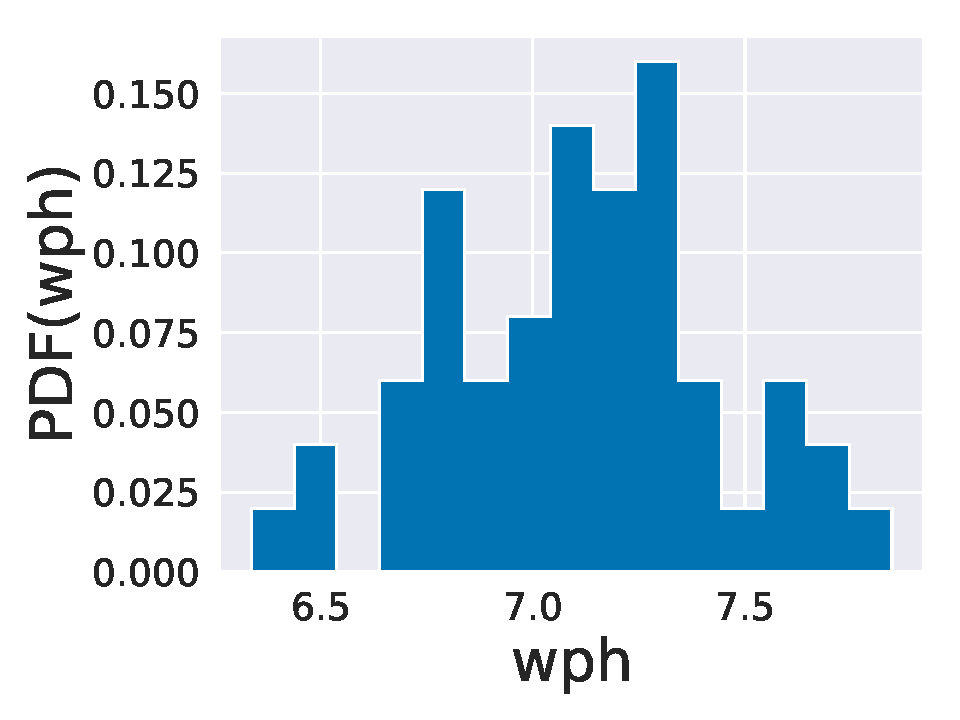
\includegraphics[width=0.32\textwidth]{slipids_20_wph}
 \caption{The probability distribution functions for each of the parametric outcomes from the Slipid potential model simulation with a effective surface pressure of \SI{20}{\milli\newton\per\meter}.}
 \label{fig:sl20}
\end{figure*}
%
%
\begin{figure*}
 \centering
 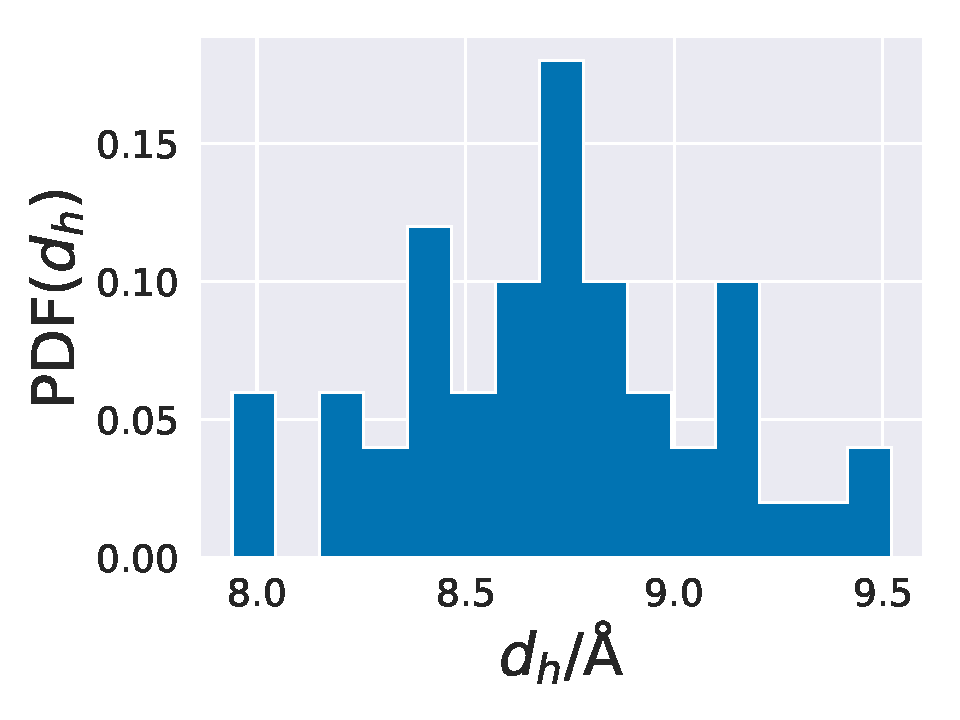
\includegraphics[width=0.32\textwidth]{slipids_30_dh}
 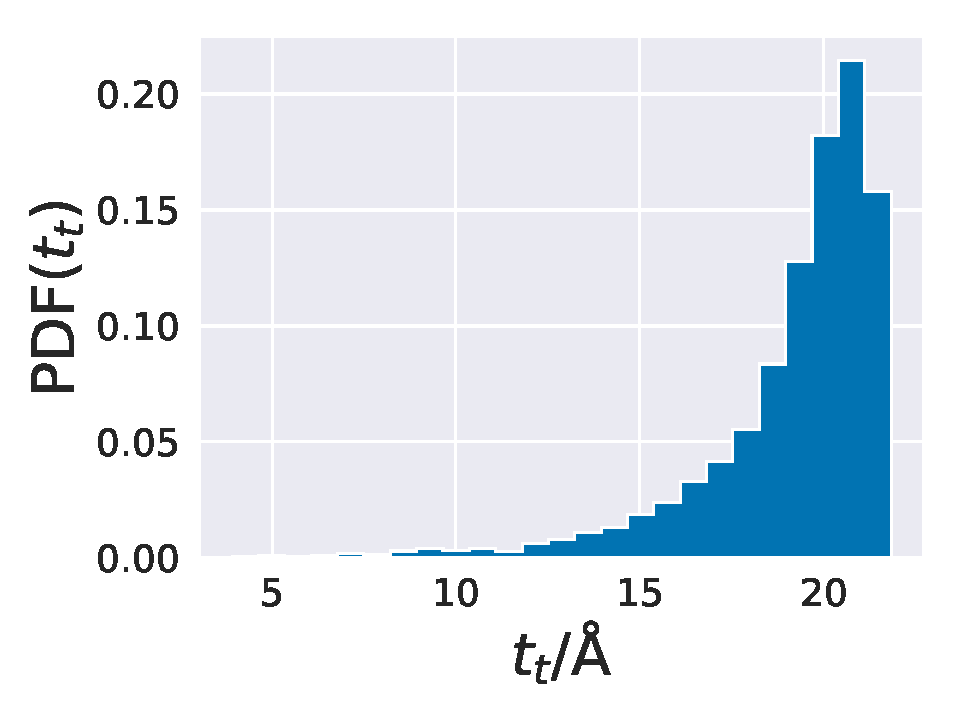
\includegraphics[width=0.32\textwidth]{slipids_30_tt}
 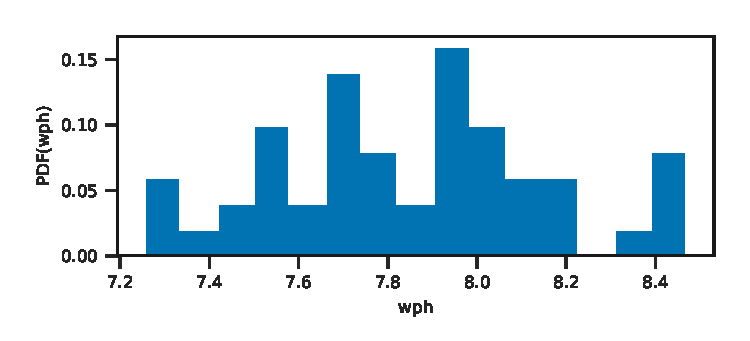
\includegraphics[width=0.32\textwidth]{slipids_30_wph}
 \caption{The probability distribution functions for each of the parametric outcomes from the Slipid potential model simulation with a effective surface pressure of \SI{30}{\milli\newton\per\meter}.}
 \label{fig:sl30}
\end{figure*}
%
%
\begin{figure*}
 \centering
 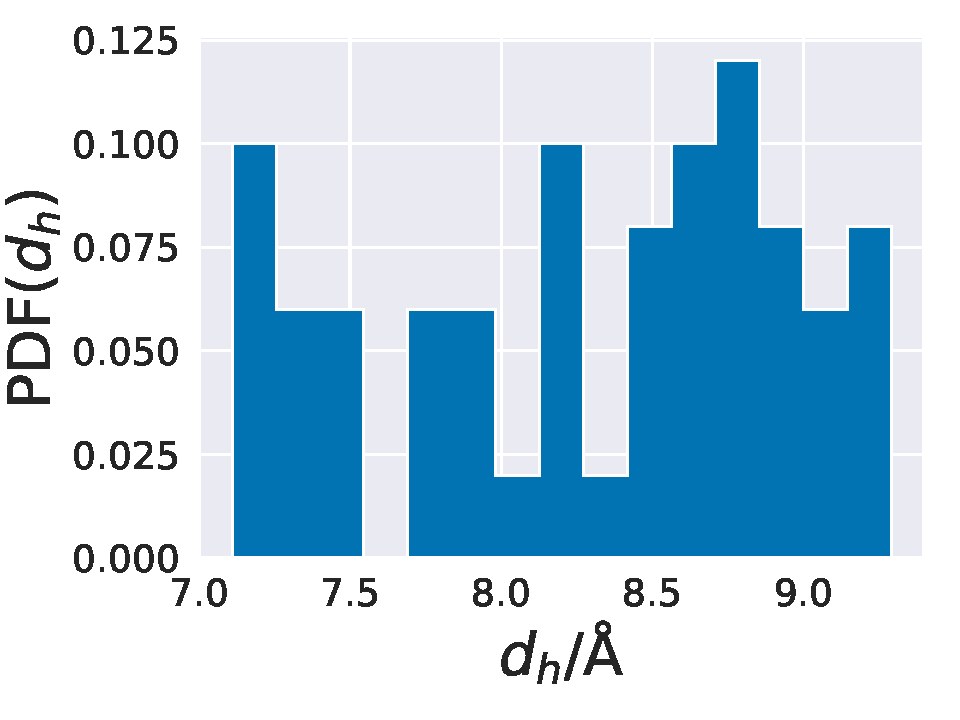
\includegraphics[width=0.32\textwidth]{slipids_40_dh}
 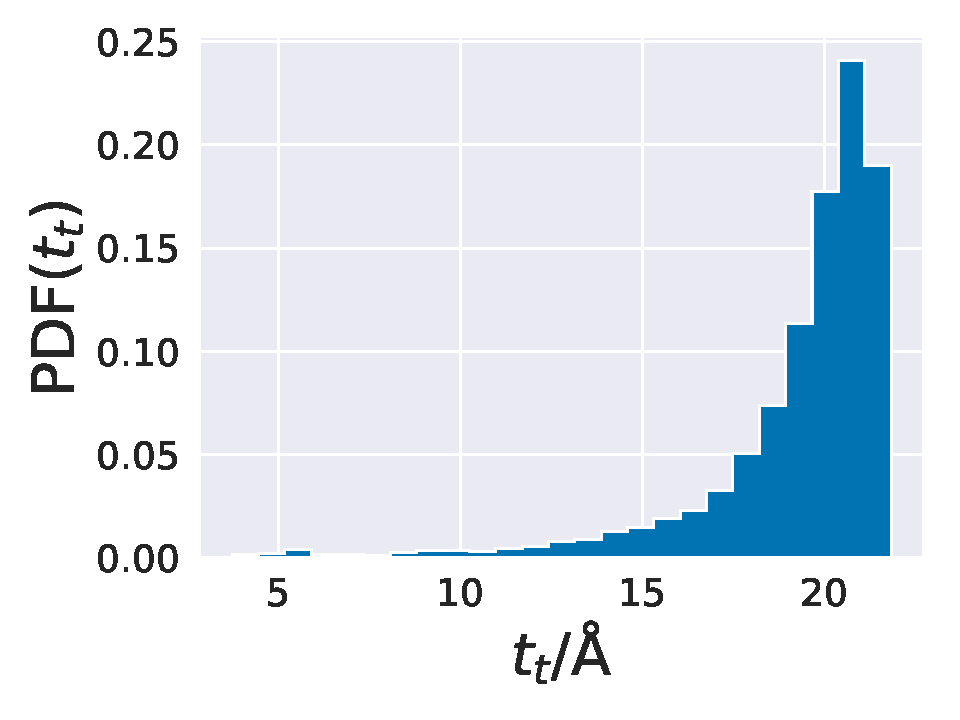
\includegraphics[width=0.32\textwidth]{slipids_40_tt}
 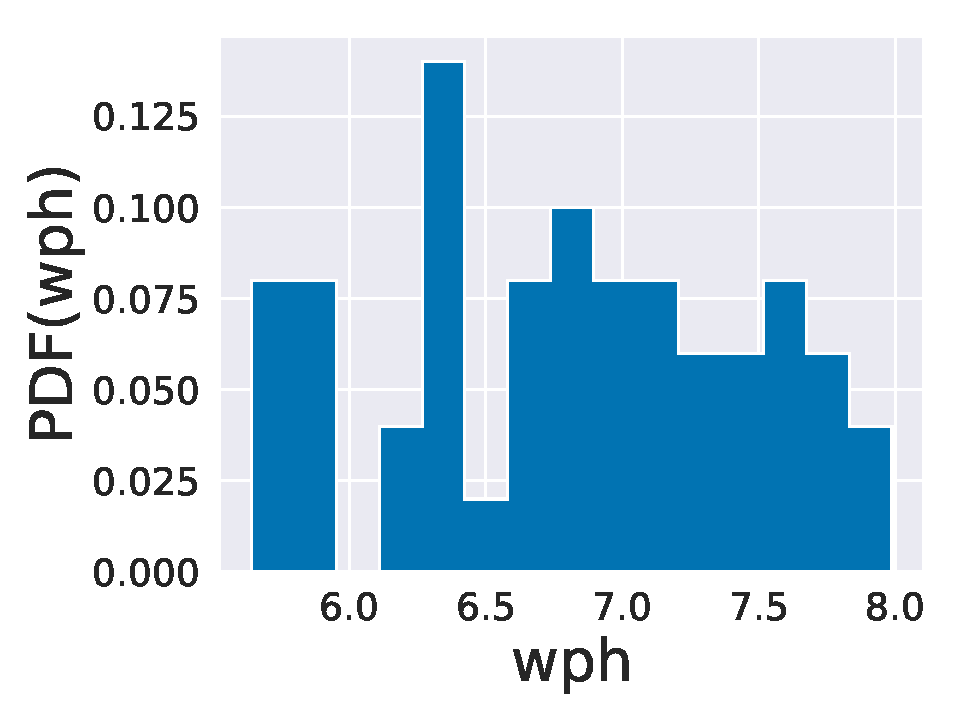
\includegraphics[width=0.32\textwidth]{slipids_40_wph}
 \caption{The probability distribution functions for each of the parametric outcomes from the Slipid potential model simulation with a effective surface pressure of \SI{40}{\milli\newton\per\meter}.}
 \label{fig:sl40}
\end{figure*}
%
%
\begin{figure*}
 \centering
 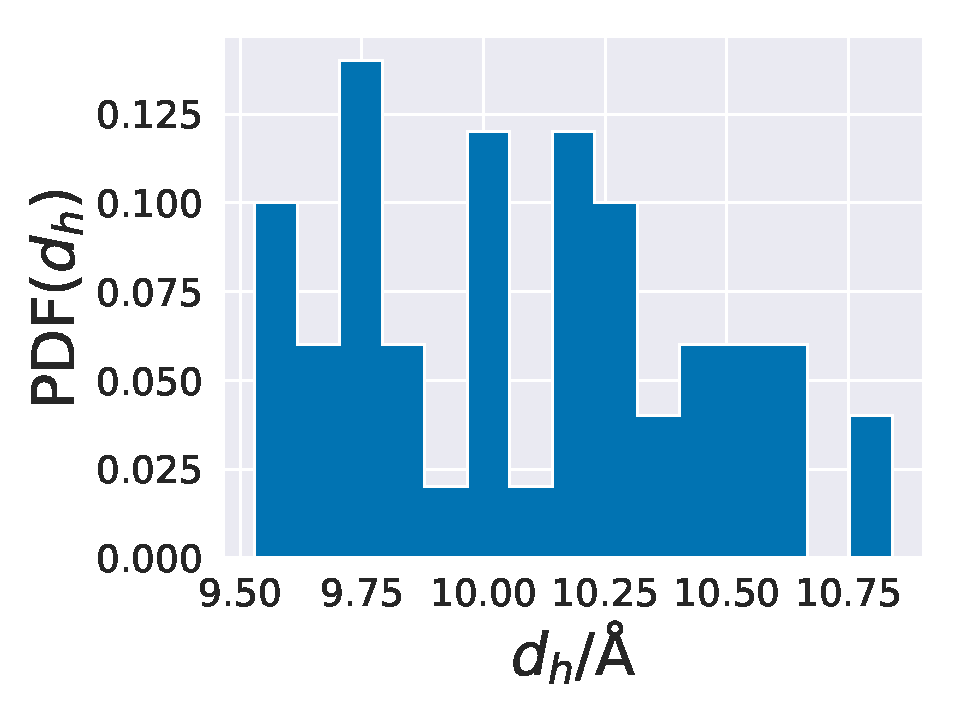
\includegraphics[width=0.32\textwidth]{slipids_50_dh}
 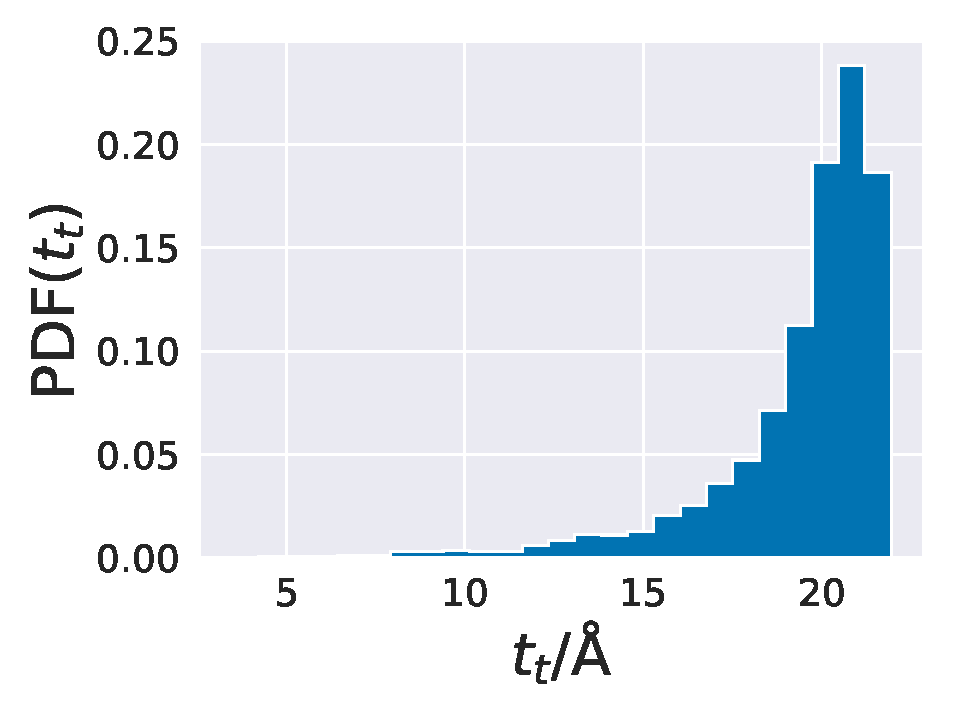
\includegraphics[width=0.32\textwidth]{slipids_50_tt}
 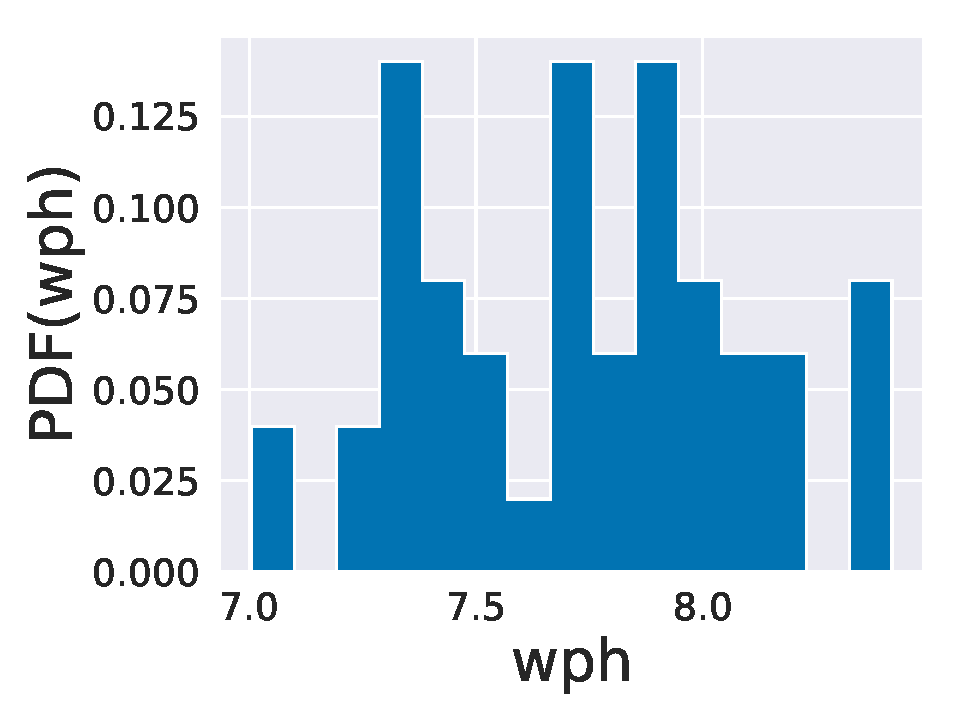
\includegraphics[width=0.32\textwidth]{slipids_50_wph}
 \caption{The probability distribution functions for each of the parametric outcomes from the Slipid potential model simulation with a effective surface pressure of \SI{50}{\milli\newton\per\meter}.}
 \label{fig:sl50}
\end{figure*}
%
%
\begin{figure*}
 \centering
 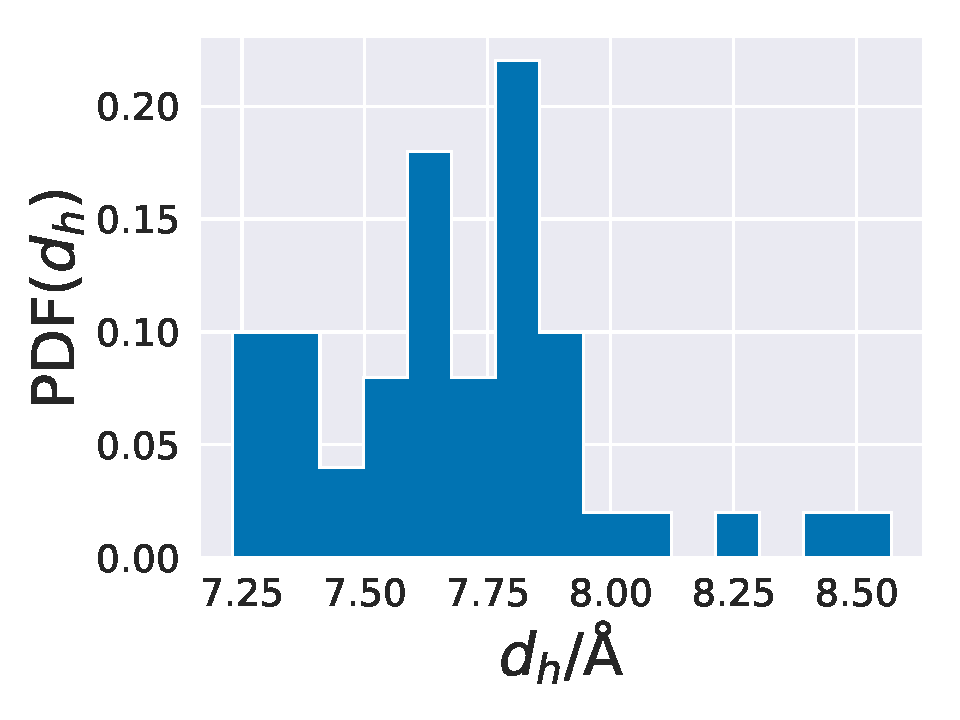
\includegraphics[width=0.32\textwidth]{berger_20_dh}
 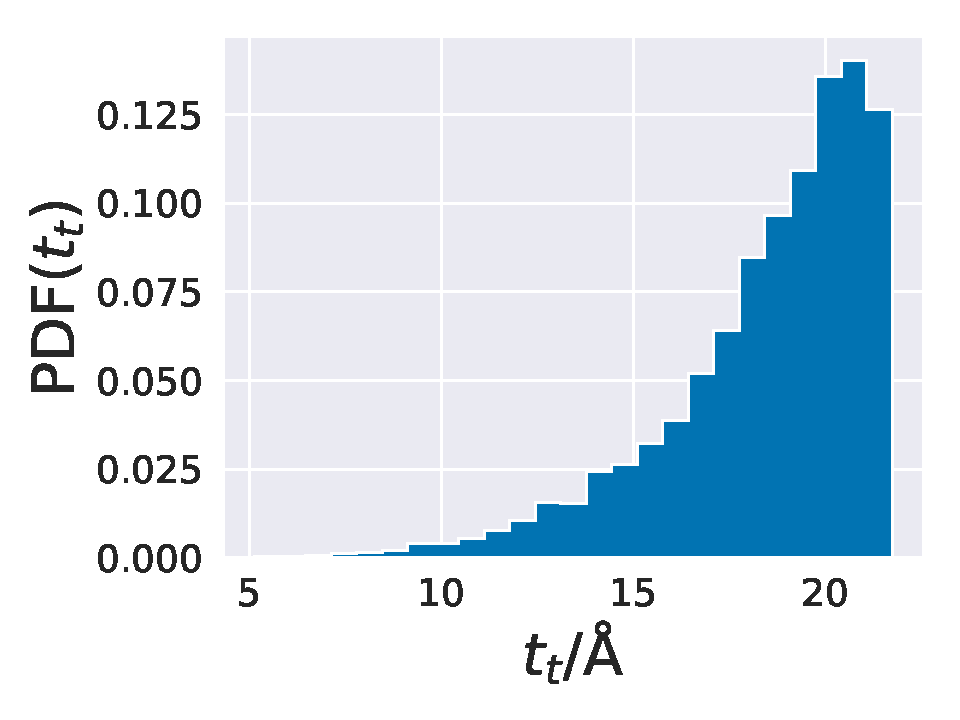
\includegraphics[width=0.32\textwidth]{berger_20_tt}
 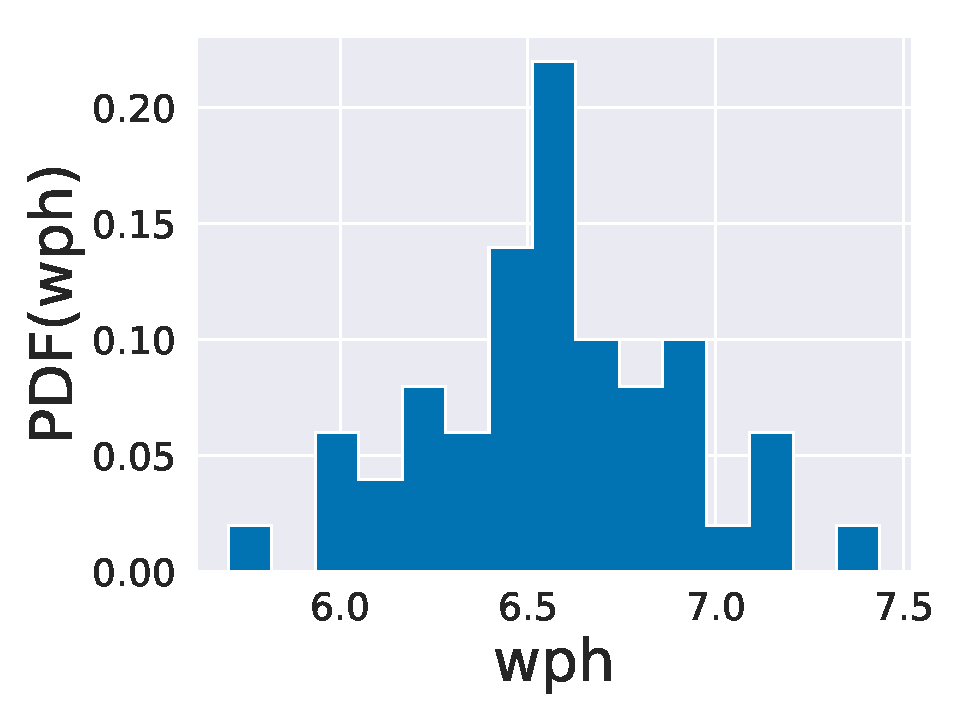
\includegraphics[width=0.32\textwidth]{berger_20_wph}
 \caption{The probability distribution functions for each of the parametric outcomes from the Berger potential model simulation with a effective surface pressure of \SI{20}{\milli\newton\per\meter}.}
 \label{fig:be20}
\end{figure*}
%
%
\begin{figure*}
 \centering
 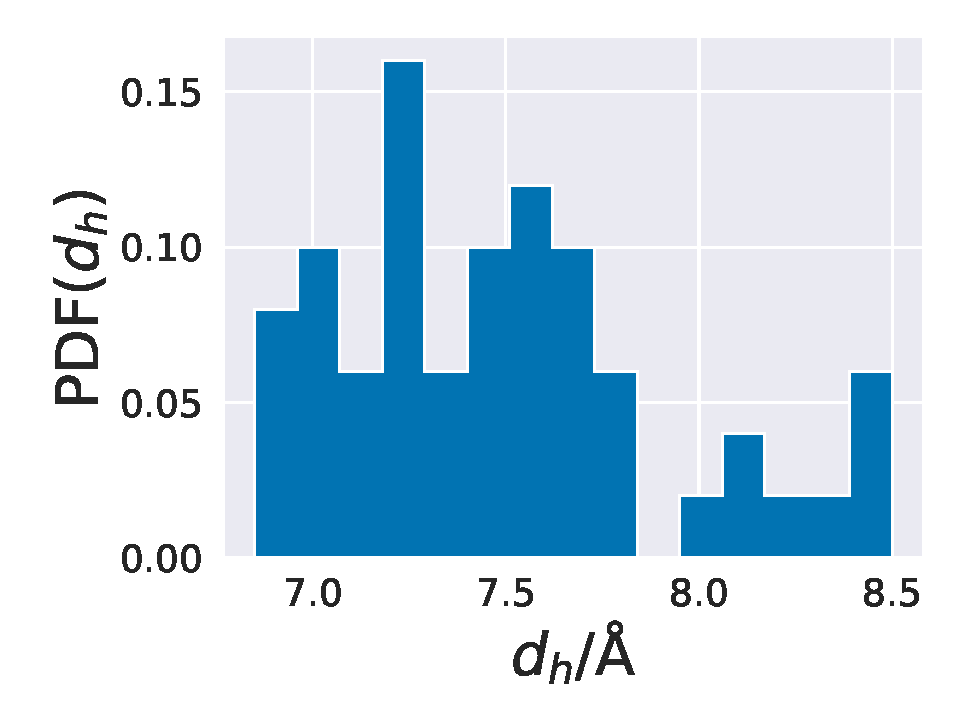
\includegraphics[width=0.32\textwidth]{berger_30_dh}
 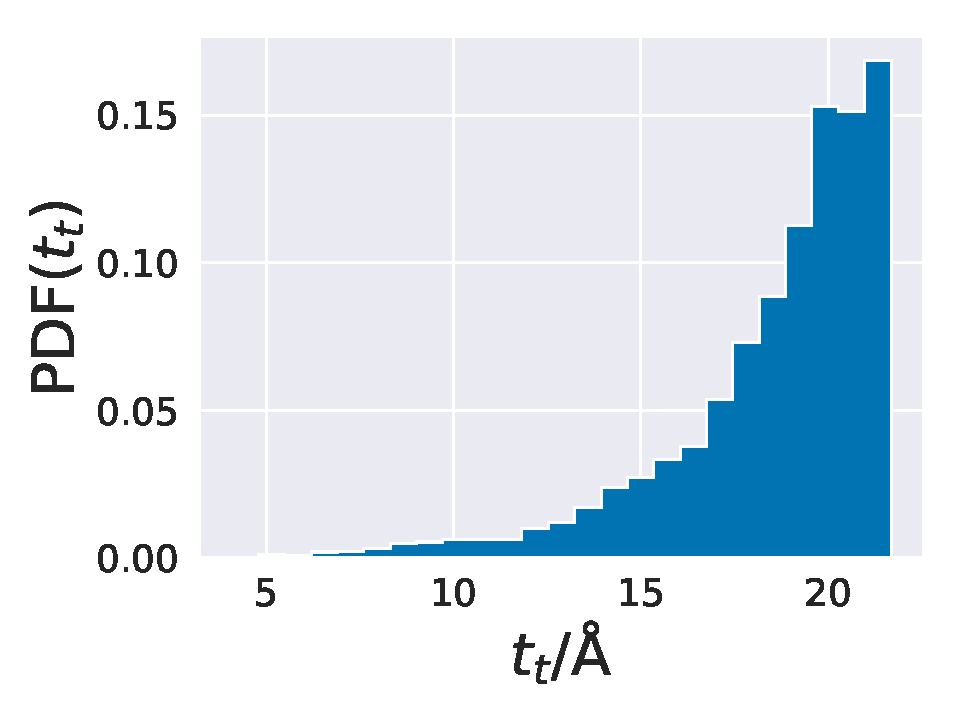
\includegraphics[width=0.32\textwidth]{berger_30_tt}
 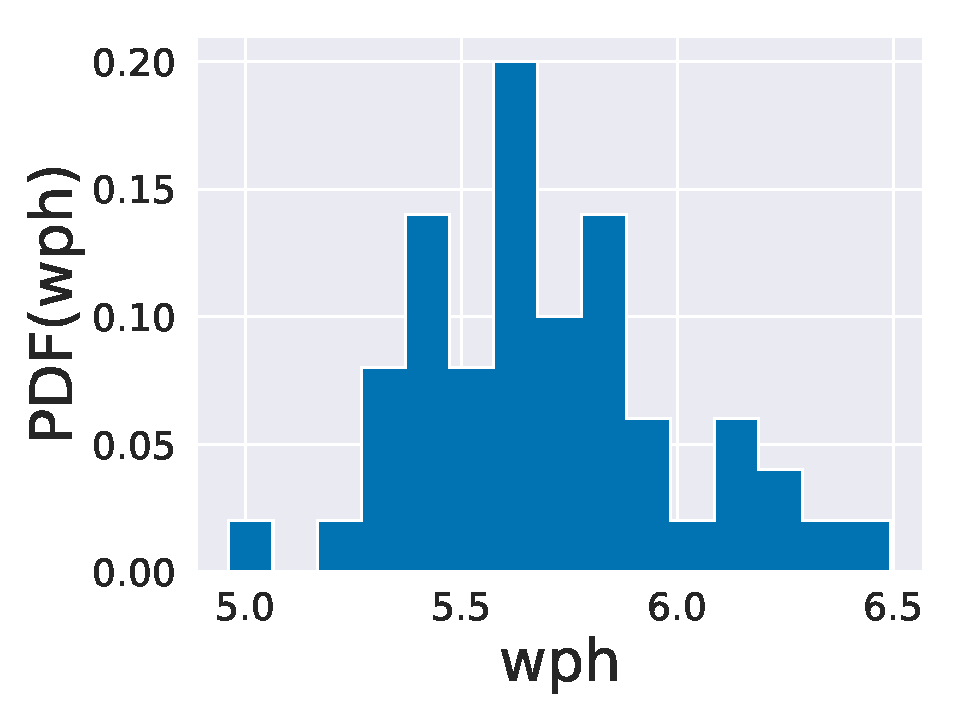
\includegraphics[width=0.32\textwidth]{berger_30_wph}
 \caption{The probability distribution functions for each of the parametric outcomes from the Berger potential model simulation with a effective surface pressure of \SI{30}{\milli\newton\per\meter}.}
 \label{fig:be30}
\end{figure*}
%
%
\begin{figure*}
 \centering
 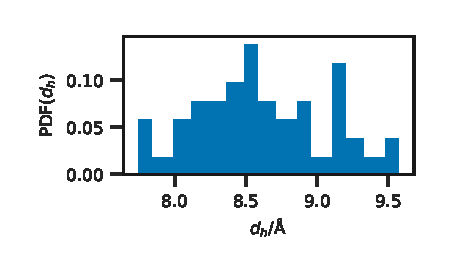
\includegraphics[width=0.32\textwidth]{berger_40_dh}
 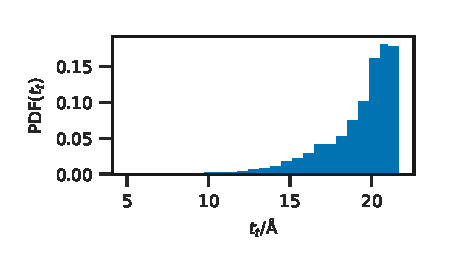
\includegraphics[width=0.32\textwidth]{berger_40_tt}
 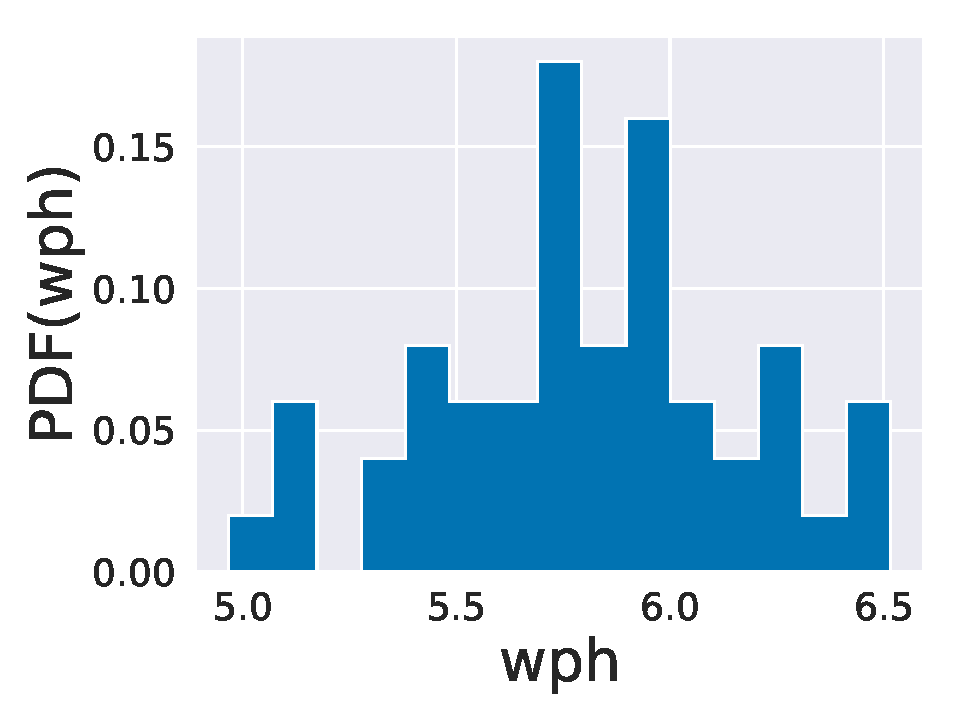
\includegraphics[width=0.32\textwidth]{berger_40_wph}
 \caption{The probability distribution functions for each of the parametric outcomes from the Berger potential model simulation with a effective surface pressure of \SI{40}{\milli\newton\per\meter}.}
 \label{fig:be40}
\end{figure*}
%
%
\begin{figure*}
 \centering
 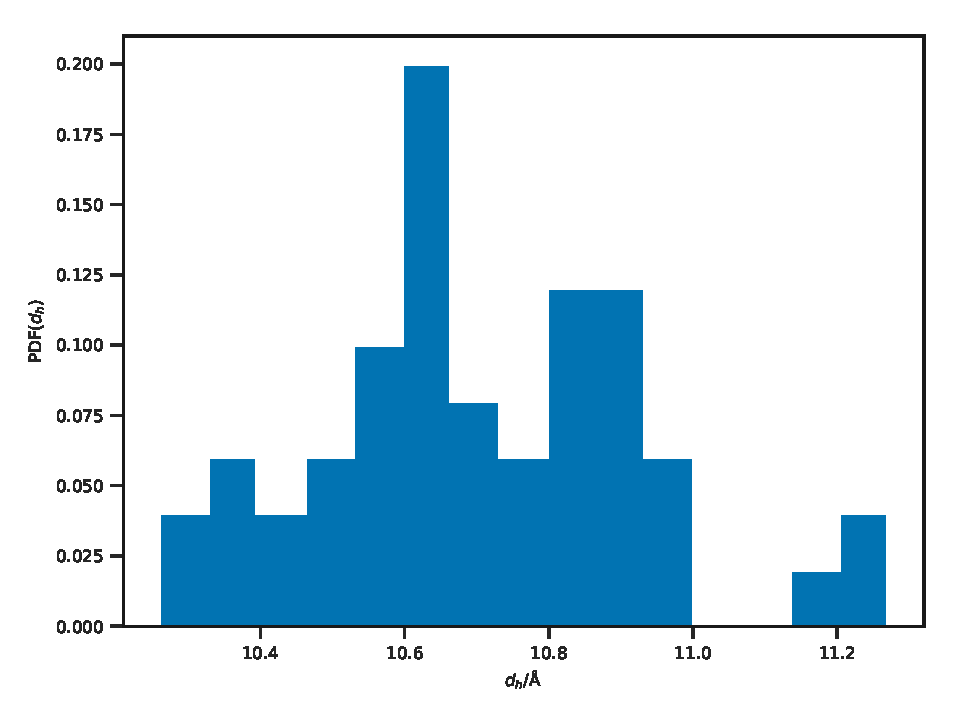
\includegraphics[width=0.32\textwidth]{berger_50_dh}
 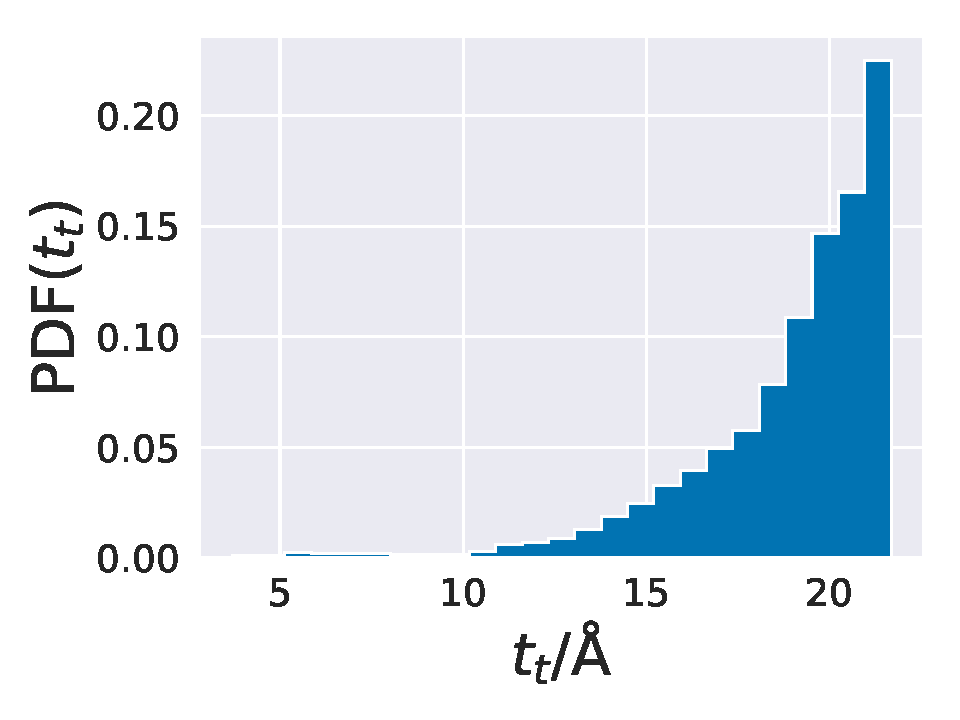
\includegraphics[width=0.32\textwidth]{berger_50_tt}
 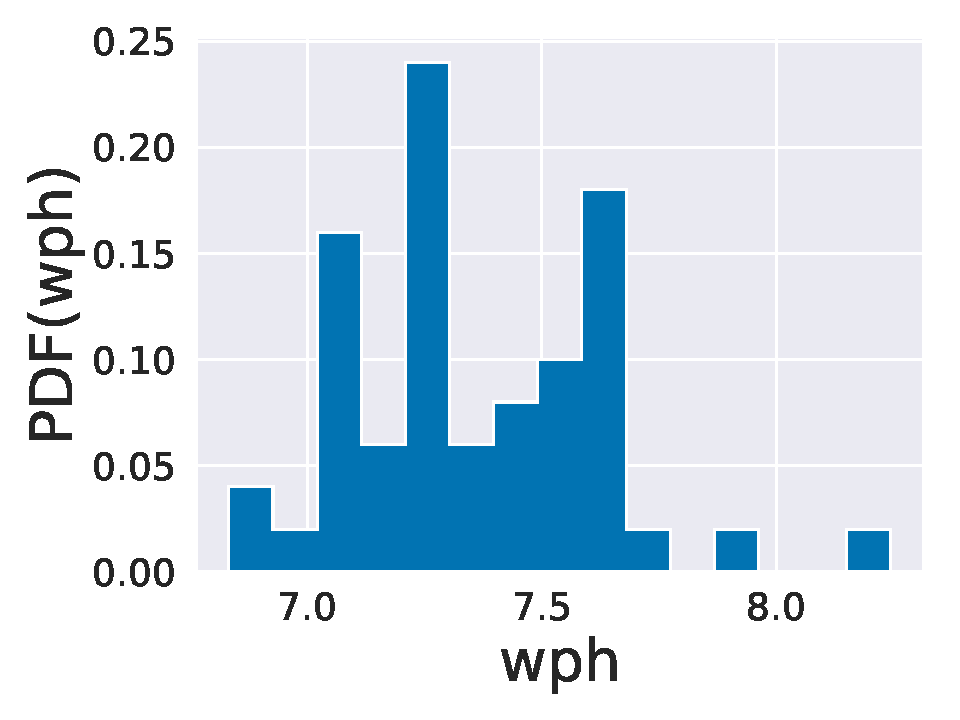
\includegraphics[width=0.32\textwidth]{berger_50_wph}
 \caption{The probability distribution functions for each of the parametric outcomes from the Berger potential model simulation with a effective surface pressure of \SI{50}{\milli\newton\per\meter}.}
 \label{fig:be50}
\end{figure*}
%
%
\begin{figure*}
 \centering
 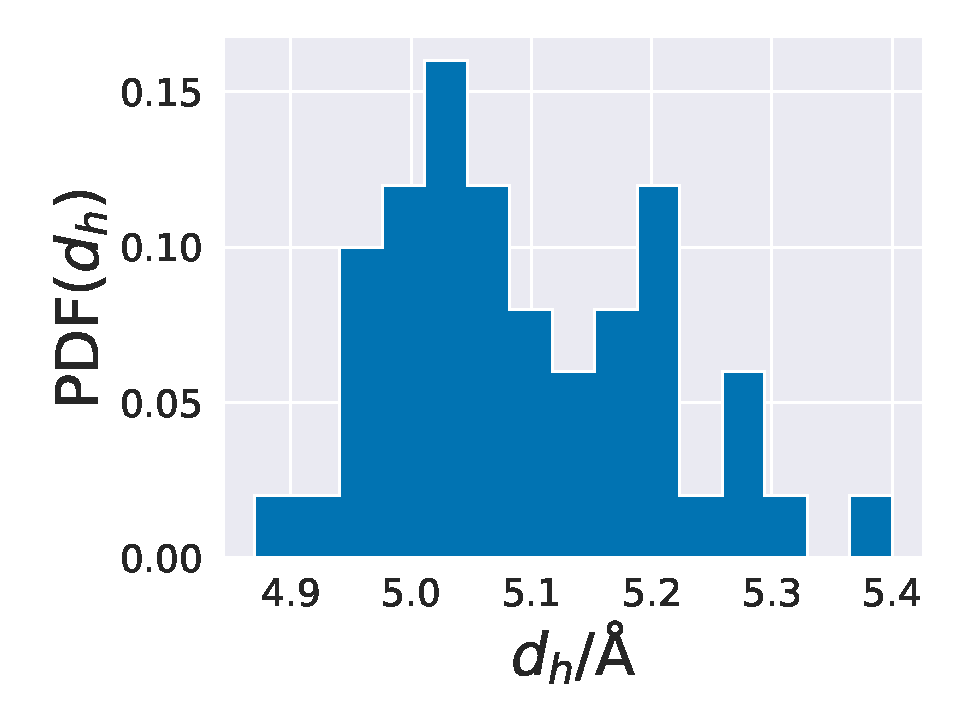
\includegraphics[width=0.32\textwidth]{martini_20_dh}
 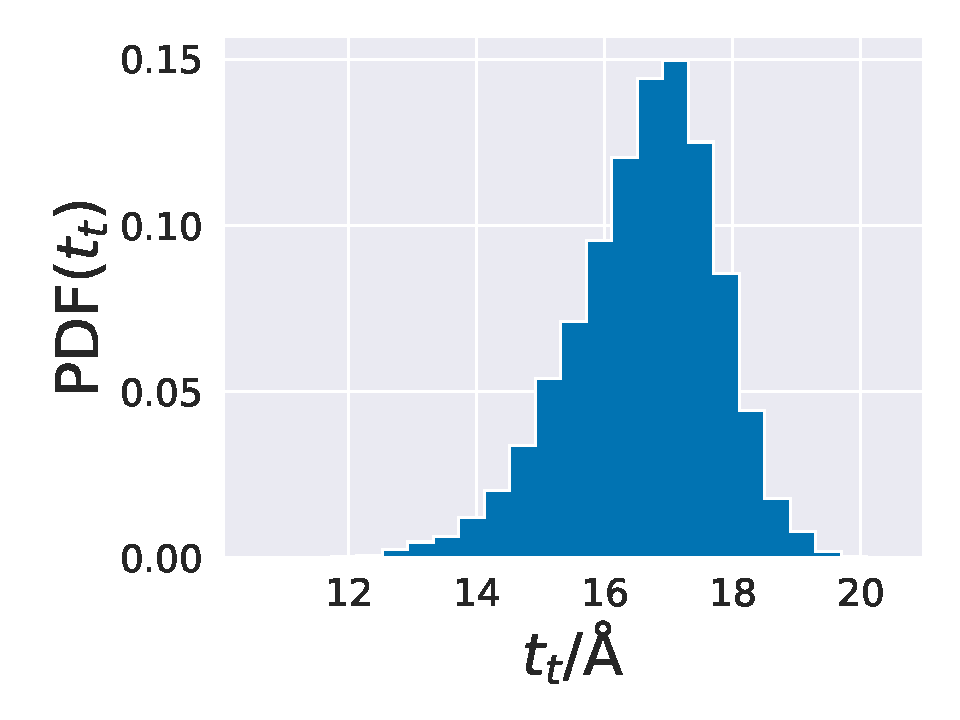
\includegraphics[width=0.32\textwidth]{martini_20_tt}
 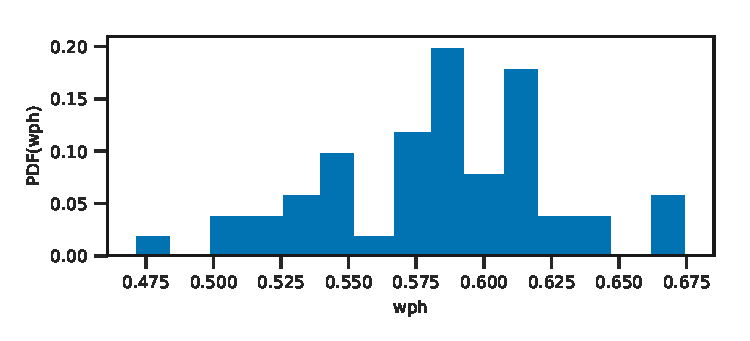
\includegraphics[width=0.32\textwidth]{martini_20_wph}
 \caption{The probability distribution functions for each of the parametric outcomes from the MARTINI potential model simulation with a effective surface pressure of \SI{20}{\milli\newton\per\meter}.}
 \label{fig:ma20}
\end{figure*}
%
%
\begin{figure*}
 \centering
 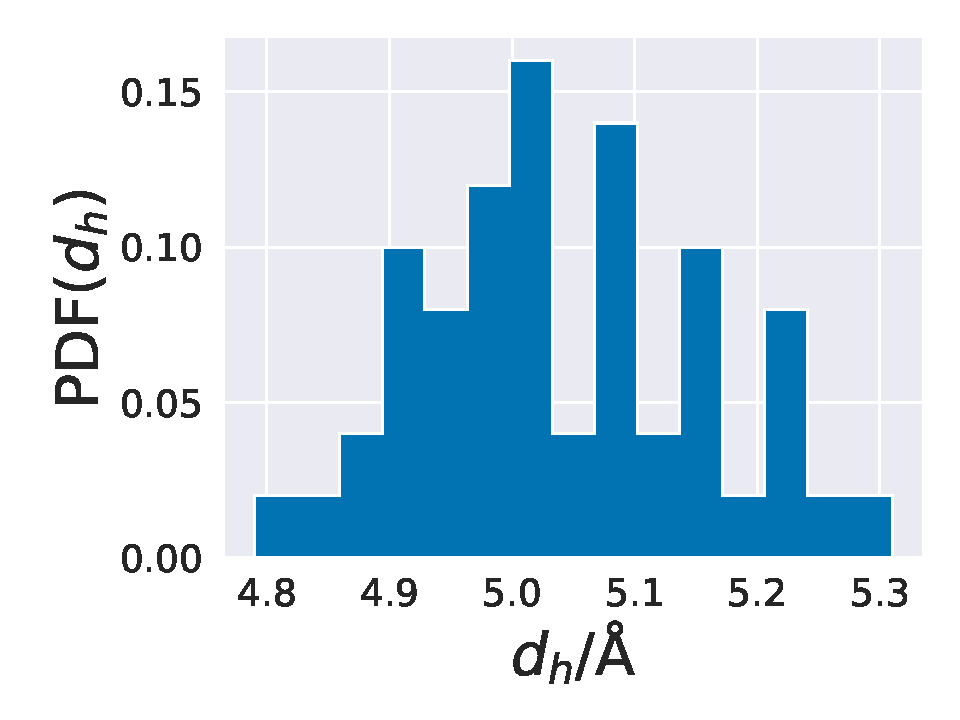
\includegraphics[width=0.32\textwidth]{martini_30_dh}
 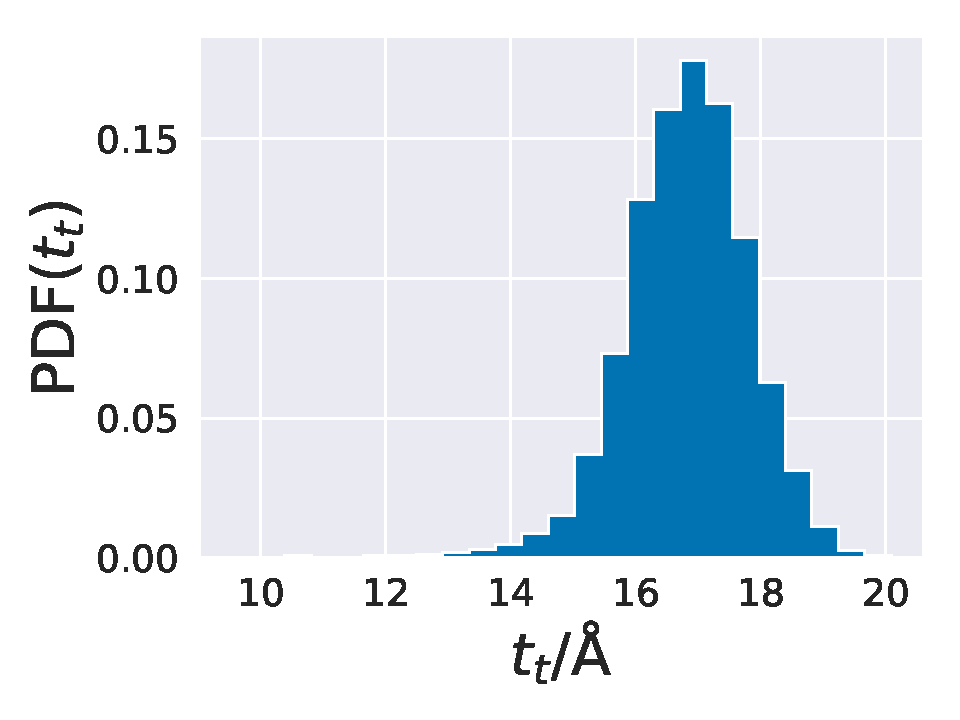
\includegraphics[width=0.32\textwidth]{martini_30_tt}
 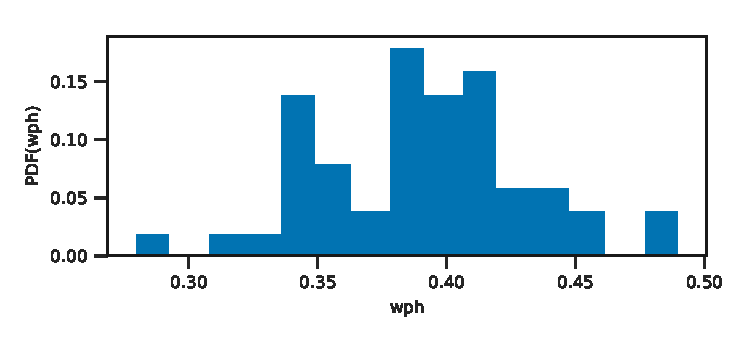
\includegraphics[width=0.32\textwidth]{martini_30_wph}
 \caption{The probability distribution functions for each of the parametric outcomes from the MARTINI potential model simulation with a effective surface pressure of \SI{30}{\milli\newton\per\meter}.}
 \label{fig:ma30}
\end{figure*}
%
%
\begin{figure*}
 \centering
 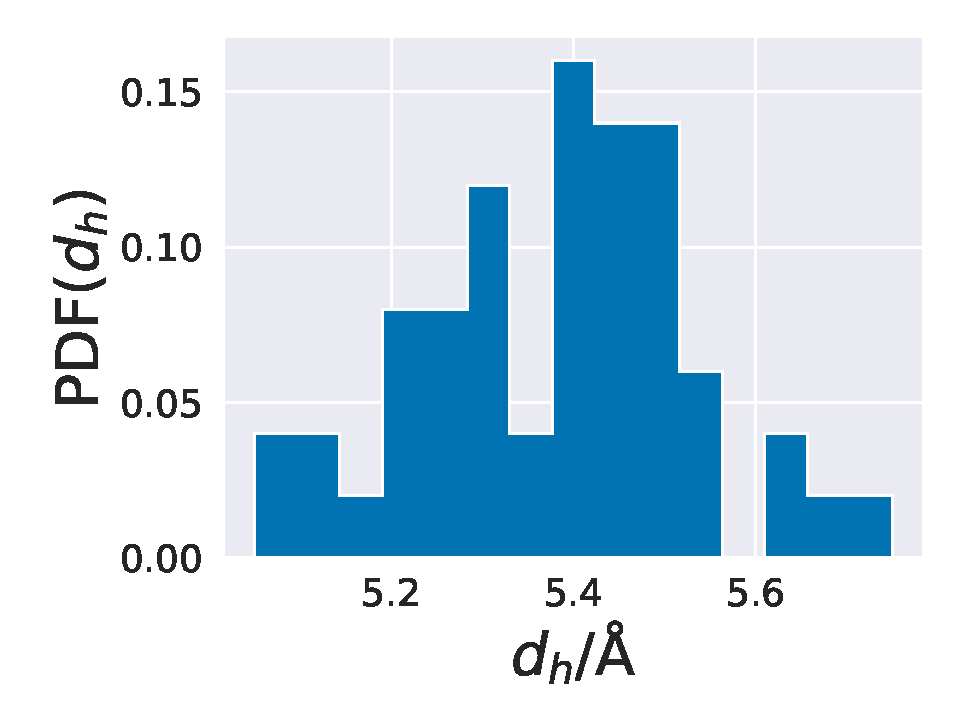
\includegraphics[width=0.32\textwidth]{martini_40_dh}
 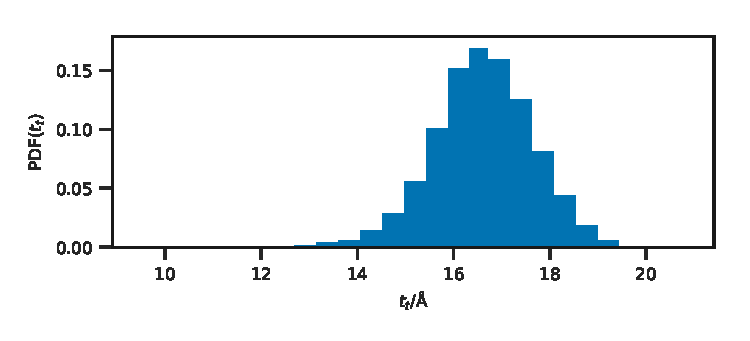
\includegraphics[width=0.32\textwidth]{martini_40_tt}
 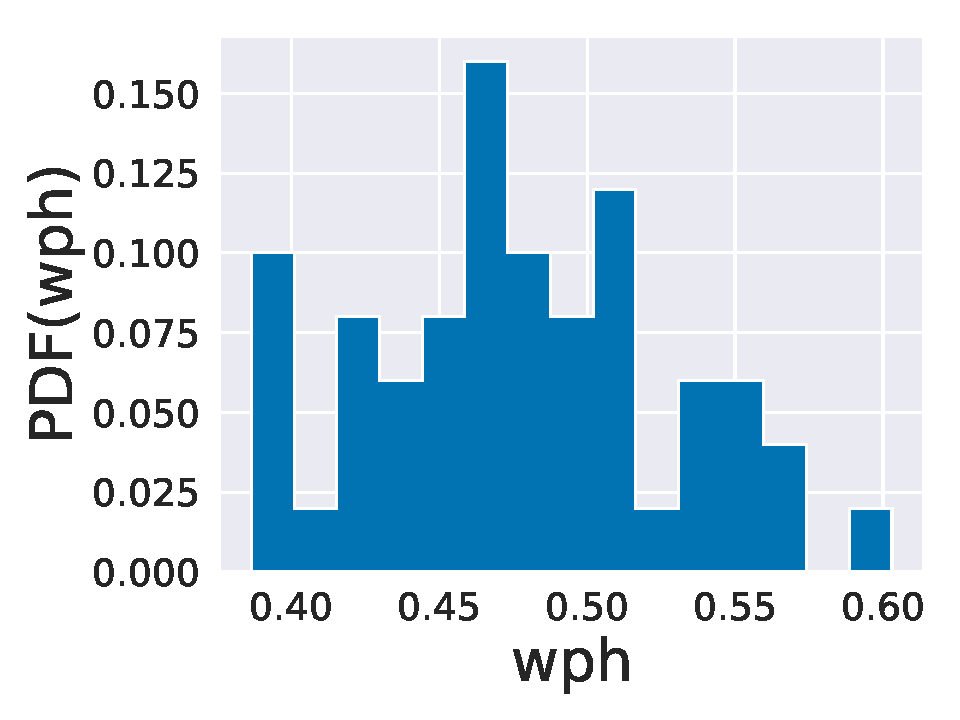
\includegraphics[width=0.32\textwidth]{martini_40_wph}
 \caption{The probability distribution functions for each of the parametric outcomes from the MARTINI potential model simulation with a effective surface pressure of \SI{40}{\milli\newton\per\meter}.}
 \label{fig:ma40}
\end{figure*}
%
%
\begin{figure*}
 \centering
 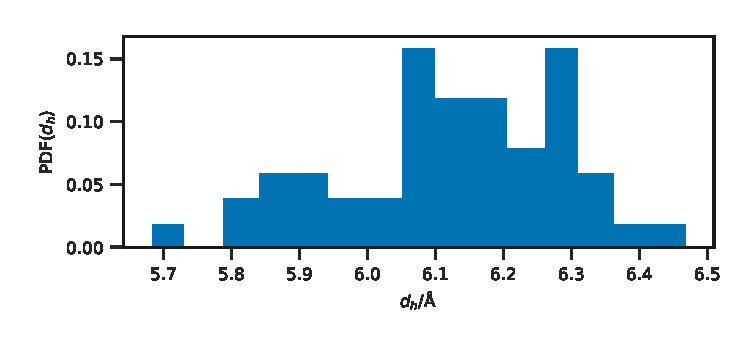
\includegraphics[width=0.32\textwidth]{martini_50_dh}
 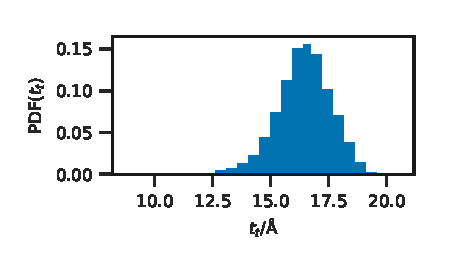
\includegraphics[width=0.32\textwidth]{martini_50_tt}
 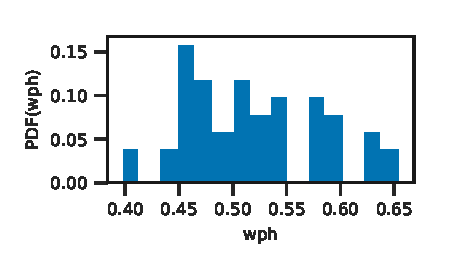
\includegraphics[width=0.32\textwidth]{martini_50_wph}
 \caption{The probability distribution functions for each of the parametric outcomes from the MARTINI potential model simulation with a effective surface pressure of \SI{50}{\milli\newton\per\meter}.}
 \label{fig:ma50}
\end{figure*}
%

\bibliography{paper.bib}


\end{document}                    % DO NOT DELETE THIS LINE
